%!TEX root = ../Masterthesis.tex
\chapter{System conception}\section{Technical conception}
\begin{figure}[H]
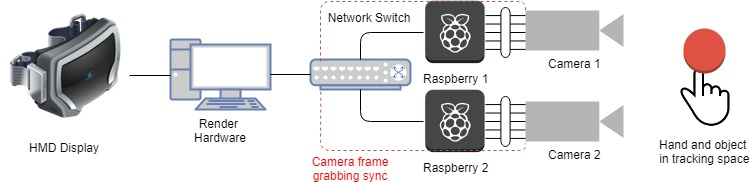
\includegraphics[width=\textwidth]{images/technical_setup.jpg}
\caption{Technical conseptiopn of the single hardware parts}
\label{technical-copnception}
\end{figure} 
The technical setup of the whole system is relatively simple. Instead of using one large dimmensioned unit which takes care of all calculations, the image processing steps that have to be done on both stereo images anyway, are outsourced onto the Raspberry Pis. As already mentioed in the conception phase, the image processing dircetly on the rapspberry also reduces latency which would occur when sending image data over network channels to the main unit.\\
The two \textbf{Raspberry Pi 3 Model B}, which are used as the controllers for the \textbf{Raspberry Pi Camera} are connected via network cable to a network switch. A connection over wireless network would be possible with the onboard capabilites of the  Pi's, but this might encounter latency problems and/or signal interference with other exisitng networks. Therefor a cable connection is the safer solution.
The switch also connects to the "Master" PC to which the "Slave" Pi's communicate their data. The Master also takes care of the stereoscopic calculations,as it is dimensioned with far more computing power than the slaves.The 2D positional data from the slaves and the calculaton results from the stereo image disparity is fed into the hand model running on the "Master". The model solution is then applied to the digital hand model and rendered to the HMD.
\section{Image Analysis with OpenCV 3 and Python on the Raspberry}
For the image analysis part, \textit{OpenCV3} with it's \textit{Python 3} bindingd is chosen. The \textit{OpenCV} package needs to be downloaded and compiled onto each device be fore it can be used.
Before the actual image anylysis part can take place, the used cameras need to be calibrated. As they are basically pinhole cameras, they introduce amounts of radial and tangetial distortion to the images. These distortions need to be compensated for, especially when using them as source for the stereo images. Image distortion in these pictures would lead to incorrect calculations for image depth.
\textit{OpenCV} supplies the tools to calculate the distortion parameters as well as the camera matrix \cite{Opencv.2018}.
The camera matrix is basically a description for the transformation of points in 3D object space to the 2D image space of the camera. For the used Cameras, we can cosinder a central projection of points in space onto our image plane. The center of the camera is considered the center of an euclidean cooridinate system and the projection plane \textbf{z} is located at distance \textit{f} equal to the focal length of the camera.\\
\begin{figure}[H]
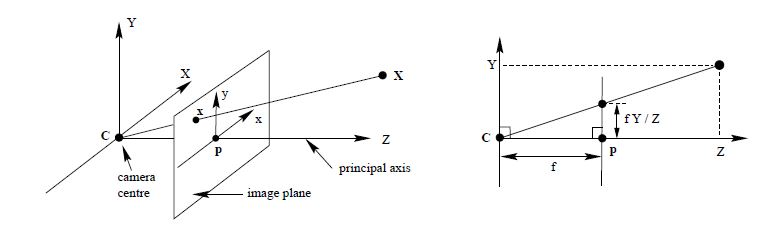
\includegraphics[width=\textwidth]{images/pionhole.JPG}
\caption{Image point projection for pinhole camera systems\cite{Hartley.2000}}
\label{pinholecamera_mapping} 
\end{figure}
As shown in Figure \ref{pinholecamera_mapping}, a point from the object space can be projected onto the image plane by drawing a ray from the onject space point to the camera center. The intersection pont of the ray with the image plane defines the projection point. With this knowledge the projection can be described as :
\begin{equation}
(X,Y,Z)^{T} \mapsto (fX/Z,fY/Z)^{T}
\end{equation}
\todo {elaborate}

For the calculation of the image distortion , \textit{OpenCv} uses a chessboard image for calibration. The printed image is held infront of the camera at a constant distance and rotated and positioned differently. After every position/rotation change an image of the pattern should be taken.
These images are then used to find the corners at the intersection of the black and white squares. With the previous knowlede of sthe square sizes, the projection errors in radial and tangential directions can be calulated:\todo{add Sourcecode}
\begin{equation}
\begin{split}
x_{tanDistorted}&=x(1+k_{1}r^{2}+k_{2}r^{4}+k_{3}+r^{6})\\
y_{tanDistorted}&=y(1+k_{1}r^{2}+k_{2}r^{4}+k_{3}+r^{6})\\
\\
x_{radDistorted}&=x+[2p_{1}xy+p_{2}(r^{2}+2x^{2})]\\
y_{radDistorted}&=x+[p_{1}(r^{2}+2y^{2})+2p_{2}xy]\\
\end{split}
\end{equation} 
As can bee seeen from the above equations, the parameters thath need to be calculated are $k_{1},k_{2},p_{1},p_{2},k_{3}$.
\todo{continue}

The python programm prototype that is used for tracking the specified color markers is comprised of the following components:
\begin{itemize}
\item Image acquisition from camera
\item Image conversion to HSV colorspace
\item Mask construction and Filtering
\item Contour finding an position calculation
\item Sending of positional data via Network as UPD Package
\end{itemize}

\subsection{Image acquisition from camera}
As the computaion times for image filtering and mask generation may vary, it makes sense to seperate the image acquisition from the computation part. Threfore the loading of the raw image data frame from the camera is outsourced into its own thread. Also this allows us to trigger the frame grabbing on both devices for synchronization. Frame grabbing synchronization is done via triggering a PWM signal on one of the raspberrys and sending it to the other Pi.
The synchronousety of the two frame reading threads is assumed for the first implementation and has to be tested on a finished setup.\\

The tread takes the data of the current image frame and hands it over to the main thread, where the image processing is handeled. For the first frames, the full image data is needed as the position of the markers is not yet known. Performancewise, this introduces a lot of overhead, since each mask generation step for the specific colors hast to go through the complete image data, meaning every pixel has to be read out at least 5 times to get the tracking for all different markers. After a few frames, we get hold of the marker position and can define a reduced region of interest (ROI) on the image. The new ROI results from the positional data from the previous frame and has to be dimmensioned correctly as to incorporate the possibility of large position differences between consecutive frames. Should no marker be found in the defined ROI or the certanty of the result is not high enough, the frame has to be dropped and the next frame should utilize the whole image data.
\subsection{Image conversion to HSV colorspace}
The image data that is supplied by the camera comes in an RGB data format, which we could already use for the further calculation. It does though make more sense to convert the imput data into the HSV colorspace. Since we are not using high precision cameras, it is necessary to define a range of color values around the desired color which we want to track. The HSV colorspace is displayed as a cone, in comparison to the RGB colorspace, which is diplayed as a cube. The color values for the HSV space are all located on a cirle spanning form 0 to 360 degrees. The Hue value (H)corresponds to the angleon the cirlce, where $0^\circ$ corresponds to a redish color, $120^\circ$ lies inthe area of green and $240^\circ$ and obove correspond to blue. The sturation value (s) coresponds to the amount of white the color contains  where 0 is pure white and 100 corresponds to the fully saturated color. For optimal results, only highly saturated colors should be used to ensure correct color detection. The last compoonent is the value component (V) which describes the intensity of the color. Alike the value settings for the saturation, value ranges of at leas 50 should be used for tracking precision.
\\
For tracking the five fingers of the hand we need five distinguishable colors. Here the primary colors red, green and blue will be the choice for the first three colors. The other two selcted colors \todo {check test results} are orange and yellow. To be able to clearly ditinguis these colors in the video frame, a constant and homogenous lighting is needed as well as a color themeprature of the lighting that is in the neutral area to not change the color of the markers.
\\the color conversion from the input RGB values to the desired HSV colorspace is done as follows:
\begin{equation}
\begin{split}
hsv_{low}=(hue_{targetcolor}-sensitivity,100,100)\\
hsv_{up}=(hue_{targetcolor}-sensitivity,100,100)\\
\end{split}
\end{equation}
\subsection{Mask construction and filtering}
\todo {orig image and mask images for display}
These values are the used as the parameters for a mask generation which generates a binary mask for the current frame where all pixels whose values lie outside of the specified range are set to zero (black) and the remaining are set to 255 (white).For these masks to work properly, any other larger objects thath might contain similar colors should be removed from the scene to eliminate worng tracking data. As all digital cameras tend to have signal noise in the sensor data , high frequenc  noise in the color channels will be present. This noise needs to be filtered out before any further computaion on the image data can be done.\\
The first step in this progress is to use a gaussian filter to blurr the mask. After this step an erosion and a dilation is applied to the image tho further eliminate unwanted noise.\todo {elaborate}
\subsection{Contour finding an position calculation}
With the cleaned mask we can continue and search for the white areas in the mask which might represent our target. Under the assumption thath we have removed all other parasitic objects from the image, the marker should be the largest area of positive pixels in the mask frame. Therefore only the largest area found in the search is taken as the desired tracking marker. For the selected area, a fitting bounding box is calculated and the center of this box is used as the positonal parameter of the tracking marker.
\subsection{Sending of positional data via network as UPD package}
The resulting data is then handed over to a seperate thread running a UDP server which sends the positional data to the parent device where the stereoscopic calulations as well as the hand model and rendering is done
\subsection{object tracking}
\todo{add object tracking method -> visual or htc vive tracker} 



 




